%!TEX root = vorlage.tex
% Martin Thoma
\section{Typical Problems in the Data for Segmentation algorithms}

Different segmentation workflows have different problems. However, there are
a couple of special cases which should get tested. Those cases might not occur
often in the training data, but it could still happen in the productive system.

\subsection{Lens Flare}
Lens flare is the effect of light getting scattered in the lens system of the
camera. The testing data set of the KITTI road evaluation
benchmark~\cite{Fritsch2013ITSC} has a couple of photos with this problem.
\Cref{fig:lens-flare} shows an extreme example of lens flare.

\subsection{Vignetting}
Vignetting is the effect of a photograph getting darker in the corners. This
can have many reasons, for example filters on the camera blocking light at the
corners.


\begin{figure}
\centering
\subfigure[Lens Flare,\newline Image by \cite{image:wikipedia:lens-flare}]{
  \label{fig:lens-flare}
  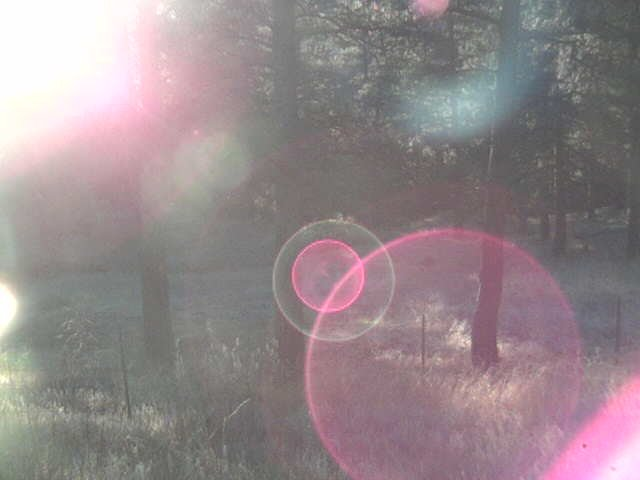
\includegraphics[width=0.45\linewidth, keepaspectratio]{figures/CCTV-Lens-flare.jpg}
}%
\subfigure[Vignetting\newline Image by \cite{image:wikipedia:vignetting}]{
  \label{fig:Vignetting}
  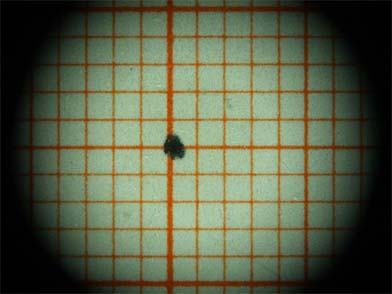
\includegraphics[width=0.45\linewidth, keepaspectratio]{figures/Randabschattung-Mikroskop-Kamera-6.JPG}
  }
\caption{Image quality problems}
\label{fig:test}
\end{figure}

\subsection{Other Problems}

\begin{itemize}
    \item reflections
    \item (Partial) occlusion
    \item Viewpoints (e.g. adult, child)
    \item Semi-Transparent objects
    \item Smoke / Foam
    \item Strong contrast on the same object, e.g. butterflies or printed
          pieces of paper
    \item Camouflage (e.g. animals like tigers in shaddow?)
    \item Group of zebras
\end{itemize}

TODO: Add some nice images
